% Created 2020-04-09 Thu 16:14
% Intended LaTeX compiler: pdflatex
\documentclass[11pt]{article}
\usepackage[utf8]{inputenc}
\usepackage[T1]{fontenc}
\usepackage{graphicx}
\usepackage{grffile}
\usepackage{longtable}
\usepackage{wrapfig}
\usepackage{rotating}
\usepackage[normalem]{ulem}
\usepackage{amsmath}
\usepackage{textcomp}
\usepackage{amssymb}
\usepackage{capt-of}
\usepackage{hyperref}
\author{Nuno Rodrigues A85207, Hugo Carvalho A85156, Hugo Ferreira A80665, João Faria A85632, João de Carvalho A83564, José Mendes A85951, José Miguel Alves Pires A50178\thanks{a50178@alunos.uminho.pt}}
\date{\today}
\title{Phase 1\\\medskip
\large Product concept, foreseen specifications, planning, tests and initial design}
\hypersetup{
 pdfauthor={Nuno Rodrigues A85207, Hugo Carvalho A85156, Hugo Ferreira A80665, João Faria A85632, João de Carvalho A83564, José Mendes A85951, José Miguel Alves Pires A50178},
 pdftitle={Phase 1},
 pdfkeywords={},
 pdfsubject={},
 pdfcreator={Emacs 26.3 (Org mode 9.3)}, 
 pdflang={English}}
\begin{document}

\maketitle
\tableofcontents

\section{Product concept}%
\label{sec:orge7b0dc6}
The envisioned product consists of a remote controlled car used to assist
exploration and maintenance domains, hereby, denominated as Radio Frequency
Camera Assisted Rover (RFCAR). To satisfy such requirements, the vehicle must
contain a remotely operated camera that provides a live video feed to the user.
Additionally, the vehicle must include an odometric system that assists the
driving and avoids unintentional collisions when remote control is compromised, e.g., when connection is lost.
The vehicle provides means for exploration and conditions assessment in critical
or unaccessible areas to human operators, such as fluid pipelines and other hazardous locations.
%
%%% Local Variables:
%%% mode: latex
%%% TeX-master: "../Phase1"
%%% End:

\section{Foreseen product specifications}
\label{sec:org31f7574}
The foreseen product specifications are listed as topics below (sketch).

\subsection{Autonomy}
\label{sec:org7364ba5}
The vehicle is operated off-the-grid, thus, a portable power source must be included. The autonomy referes to the time interval between battery fully charged and safely discharged and should be observed for the following scenarios:
\begin{itemize}
\item No load;
\item Vehicle operating at maximum speed;
\item Vehicle operating at minimum speed.
\end{itemize}
\subsection{Velocity}
\label{sec:org08718bc}
The velocity the car achieves is determined by the voltage of the motors, allowing to operate the car at the desired velocity simply varying the dutycicle of the control signal to the motors. The maximum velocity is achieved when the dutycicle of all motor control signals are 1 and the car does not have any load. 
\subsection{Safety}
\label{sec:org83942c3}
For a remote controlled car, safety concerns not only the car itself and all of the equipment, but also the humans that interact with the car:
\begin{itemize}
\item Car: If the user issues a command that would cause damage to the system, the
system should take corrective measures to prevent it. The same holds true if
the communication between user and system is lost.
\begin{itemize}
\item \textbf{System uses odometric navigation}
\end{itemize}
\item Human: Due to the odometric sensors safely fixed in the car, crashes will not occur, making it much harder for the car to hit a person or for any part of the car to jump and cause harm to the user or anyone around.
\end{itemize}
\subsection{Image acquisition}
\label{sec:orgb6a5f66}
\subsubsection{Frame rate}
\label{sec:org5adf4ee}
Frame rate refers to the frequency at which independent still images appear on the screen. The higher the frame rate, a better image quality is obtained but the processing overhead increases as well, so a compromise must be achieved between the quality of the image and the processing overhead required.
\subsubsection{Range}
\label{sec:orgecb044c}
How far can the camera capture images without loosing resolution and record them.
\subsubsection{Resolution}
\label{sec:orgba87554}
The amount of detail that the camera can capture. It is measured in pixels. The quality of the aquired image is proportional to the number os pixels but a greater resolution requires a greater data transfer and processing overhead, thus, a compromise must be achieved.
\subsubsection{Color scale (Black and white or color)}
\label{sec:org468ee04}
É preciso estar aqui isto ?
\subsubsection{Always present or enabled on user command}
\label{sec:orgd585352}
É preciso estar aqui isto ?
\subsection{Usability}
\label{sec:org61632e0}
\begin{itemize}
\item User-friendly interface
\item User interface responsiveness
\end{itemize}
\subsection{Load}
\label{sec:orgca6a690}
The remote control car can be used 
\subsection{Overall System latency/responsivess}
\label{sec:org7fd1829}
The overall system latency is the sum of all systems' latencies, which must be
under a maximum tolerated value for the user.
\subsection{Communication}
\label{sec:org4241610}
\subsubsection{Reliability}
\label{sec:orgdcb920d}
Packet must be delivered (reliable, e.g. TCP) or not (e.g. UDP)
\subsubsection{Range}
\label{sec:org447a205}
The communication protocols have a limited range of operation, and, as such, regarding the environment on which the car is used the range can be changed.
The range refers to the maximum distance allowed between user and system for communication purposes.
\subsubsection{Transmission rate / throughput}
\label{sec:org10e75a5}
\subsubsection{Redundancy}
\label{sec:orgc5933fc}
The communication protocols are not flawless and the car relies on them to be controlled. If the communication is lost, the car cannot be controlled. A possible solution for this issue is using more communication protocols (e.g Wi-fi and bluetooth), so when one protocol fails, the car can still be controlled by the other.
\subsection{Sensibility}
\label{sec:org622e63a}
The movement of the car will be determined by the tilt movement of the smartphone. Sensibility refers to the responsiveness of the car on the minimum smartphone tilt movement.
\subsubsection{Msg Smartphone->Raspberry}
\label{sec:org6b5cb97}
x10 y20 v10
t5 v5

\noindent\rule{\textwidth}{0.5pt}
\subsection{Closed loop error (Control team)}
\label{sec:org436f732}
The closed loop control assures that upon the loss of communication or a command from the user that can cause harm to the car or anyone, the car will not crash. To do so, the velocity, direction and distance to objects must be controlled. The control consists on the comparation of the desired position with the current position, thus generation the error.
\subsubsection{PI}
\label{sec:org9859444}
\subsubsection{PID}
\label{sec:org352c4d4}
\subsubsection{PD}
\label{sec:org0d324c4}

\subsection{Summary}
\label{sec:org1f95256}
Table \ref{tab:specs-init} lista the foreseen product specifications.

% Please add the following required packages to your document preamble:
\begin{table}[!hbt]
\centering
\caption{Specifications}
\label{tab:specs-init}
\resizebox{\textwidth}{!}{%
\begin{tabular}{lll}
\hline
 & Values & Explanation \\ \hline
Max Velocity & 0.2 m/s & Maximum velocity of the conveyor belt in steady state \\ \hline
Dimensions & 60x30x30 cm & Dimensions of the conveyor belt in cm {[}l w h{]} \\ \hline
Time Min & 3 s & \begin{tabular}[c]{@{}l@{}}Time taken to transport a load the full extent \\ of the conveyor belt at maximum velocity\end{tabular} \\ \hline
Max Load & 1 Kg & \begin{tabular}[c]{@{}l@{}}Load the belt can hold without causing any \\ harm to the product\end{tabular} \\ \hline
Max slope & 15$^\circ$ & \begin{tabular}[c]{@{}l@{}}Maximum slope in which the conveyor belt can \\ operate at nominal conditions\end{tabular} \\ \hline
Slope levels & {[}0,5,10,15{]}$^\circ$ & Different levels of slope manually handled \\ \hline
Settling time & 0.2 $\cdot$ T & \begin{tabular}[c]{@{}l@{}}This means that it takes up to 20\% of the full \\ travel time to reach steady velocity\end{tabular} \\ \hline
Overshoot & 110\% Vss & \begin{tabular}[c]{@{}l@{}}Maximum velocity the conveyor belt reaches \\ before settling time\end{tabular} \\ \hline
Margin of error & 95\%-105\% of Vss & Admissible error in steady velocity \\ \hline
Power supply & 12V batteries, 6W & The main power supply will be 12V batteries \\ \hline
\end{tabular}%
}
\end{table}

%%% Local Variables:
%%% mode: latex
%%% TeX-master: "../Phase1"
%%% End:

%\section{Planning}%
%\label{sec:orga82318d}
In fig.~\ref{fig:gantt-diag-orig} is illustrated the Gantt chart for the project, containing the tasks' descriptions. It should be noted
that the project tasks of Analysis, Design, Implementation and Tests are
performed in two distinct iterations as corresponding to the Waterfall project
methodology.

Due to unpredictable circumstances, limiting the mobility of team
staff and goods, the implementation stage will not be done at full extent, but
rather at a simulation stage. Thus, to overcome these constraints, the project
focus is shifted to the simulation stage, where an extensive framework as to
built to model the system operation, test it, and providing valuable feedback
for the dependents modules. As an example, the modules previously connected just
by an RS232 link, must now include upstream a web module (TCP/IP) --- the data
is now effectively sent through the internet, and must be unpacked and delivery
serially as expected if only the RS232 link was used.

The tasks are described as follows:
\begin{itemize}
\item \uline{Project Kick-off}: in the project kick-off, the group is formed and the tutor
is chosen. A brainstorming about conceivable devices takes place, whose
viability is then assessed, resulting in the product concept definition
(Milestone 0).
\item \uline{State of the Art}: in this stage, the working principle of the device is
studied based on similar products and the system components and its
characteristics are identified.
\item \uline{Analysis}: In the first stage --- Analysis 1 --- contains the analysis
results of the state of the art. It should yield the specifications document,
containing the requisites and restrictions to the project/product, on a
quantifiable basis as required to initiate the design; for example, the
vehicle's desired speed should be, at maximum, \texttt{2 m/s}. The second stage --- Analysis 2
--- contains the analysis of the first iteration of the development cycle.
\item \uline{Design}: it is done in two segments: modules design --- where the modules are
designed; integration design --- where the interconnections between modules is
designed. It can be subdivided into \emph{conceptual design} and \emph{solution
design}. 
\begin{itemize}
\item In the conceptual design, several problem solutions are identified,
quantifying its relevance for the project through a measuring scale,
inserted into an evaluation matrix, for example, QFD.%
\item In the solution design, the selected solution is developed. It must include
the solution modelling, e.g.:
\begin{itemize}
\item \uline{Control system}: analytically and using simulation;
\item \underline{Transducer design}: circuit design and simulation;
\item \uline{Power system}: power supply, motors actuation and
  respective circuitry design and simulation;
\item \uline{Communications middleware}: communication protocols evaluation and
  selection;
\item \uline{Software layers}: for all required modules, and considering its
  interconnections, at distinct levels:
  \begin{itemize}
  \item \uline{front end layer}: user interface software, providing a easy and convenient
    way for the user to control and manage the system.
  \item \uline{framework layer}: software required to emulate/simulate and test the
    required system behaviour, providing seamless interfaces for the dependents
    modules
  \item \uline{back end layer}: software running \emph{behind the scenes}, handling user
    commands received, system monitoring and control.
  \end{itemize}
\end{itemize}
\end{itemize}
\item \uline{Implementation}: product implementation which is done by
  \uline{modular integration}. In the first stage, the implementation is done in a prototyping
environment --- the assisting framework developed, yielding version alpha; in the second stage
it must include the coding on the final target modules, yielding
prototype beta.
\item \uline{Tests}: modular tests and integrated tests are performed. Tests are generally considered as those performed over any physical
component or prototype. Here, it is used as a broader term, to reflect the tests
conducted into the system and the several prototypes.
\item \uline{Functional Verification/Validation}: System verification may be performed to validate overall
  function, but not for quantifiable measurement, due to the latencies
  involved. Regarding validation, specially for an external agent, thus, it should be limited
  to user interface validation.
\item \uline{Delivery}: --- project closure encompassing:
\begin{enumerate}
\item Final prototype
\item Support documentation: how to replicate, instruction manual.
\item Final report
\item Public presentation
\end{enumerate}
\end{itemize}
%
%%%%%%%%%%%%%%% Figure is deprecated: use PDF instead
%\begin{figure}[!htbp]
%\centering
%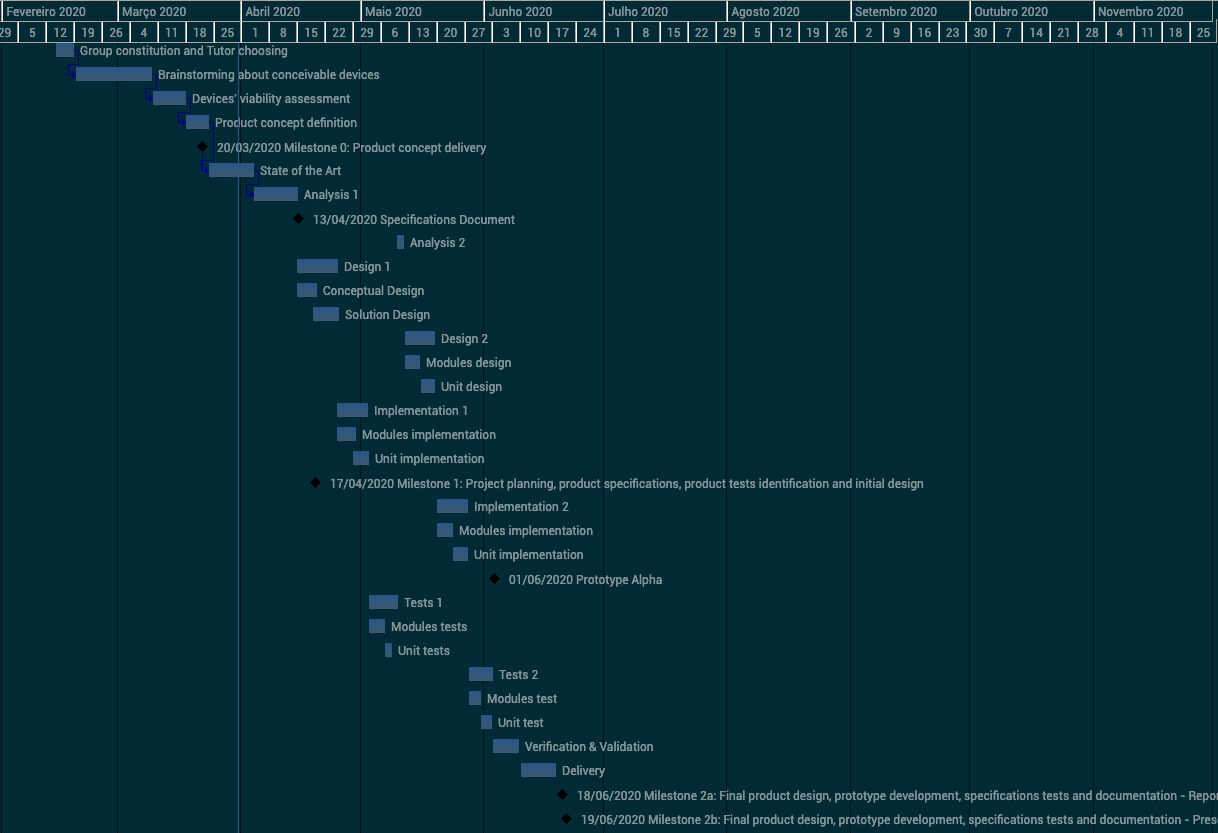
\includegraphics[width=1.0\textwidth]{./sec/img/gantt-diag-orig.png}
%\caption{\label{fig:gantt-diag2}Project planning: Gantt diagram 1}
%\end{figure}
%\begin{figure}[!htbp]
%\centering
%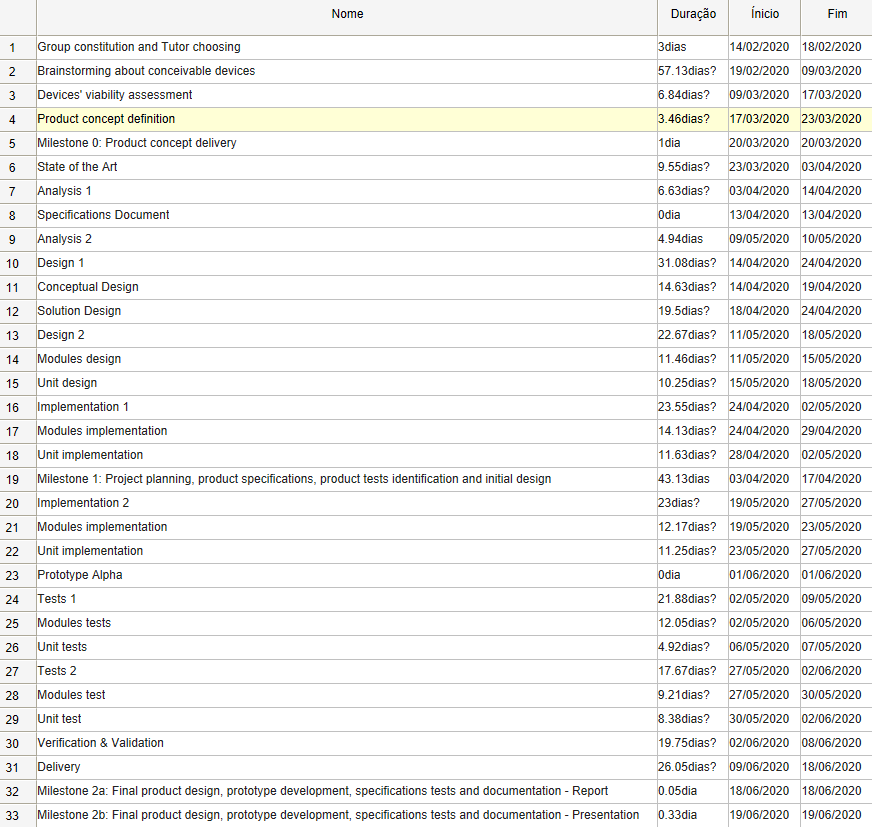
\includegraphics[width=1.0\textwidth]{./sec/img/gantt-orig-tasks.png}
%\caption{\label{fig:gantt-tasks}Project planning: tasks}
% \end{figure}
%%%%%%%%%%%%%%%%%%%%%%%%%%%%%%%%%%%%%%%%%%%%%%%%%%%%%%%%%%%%%
% 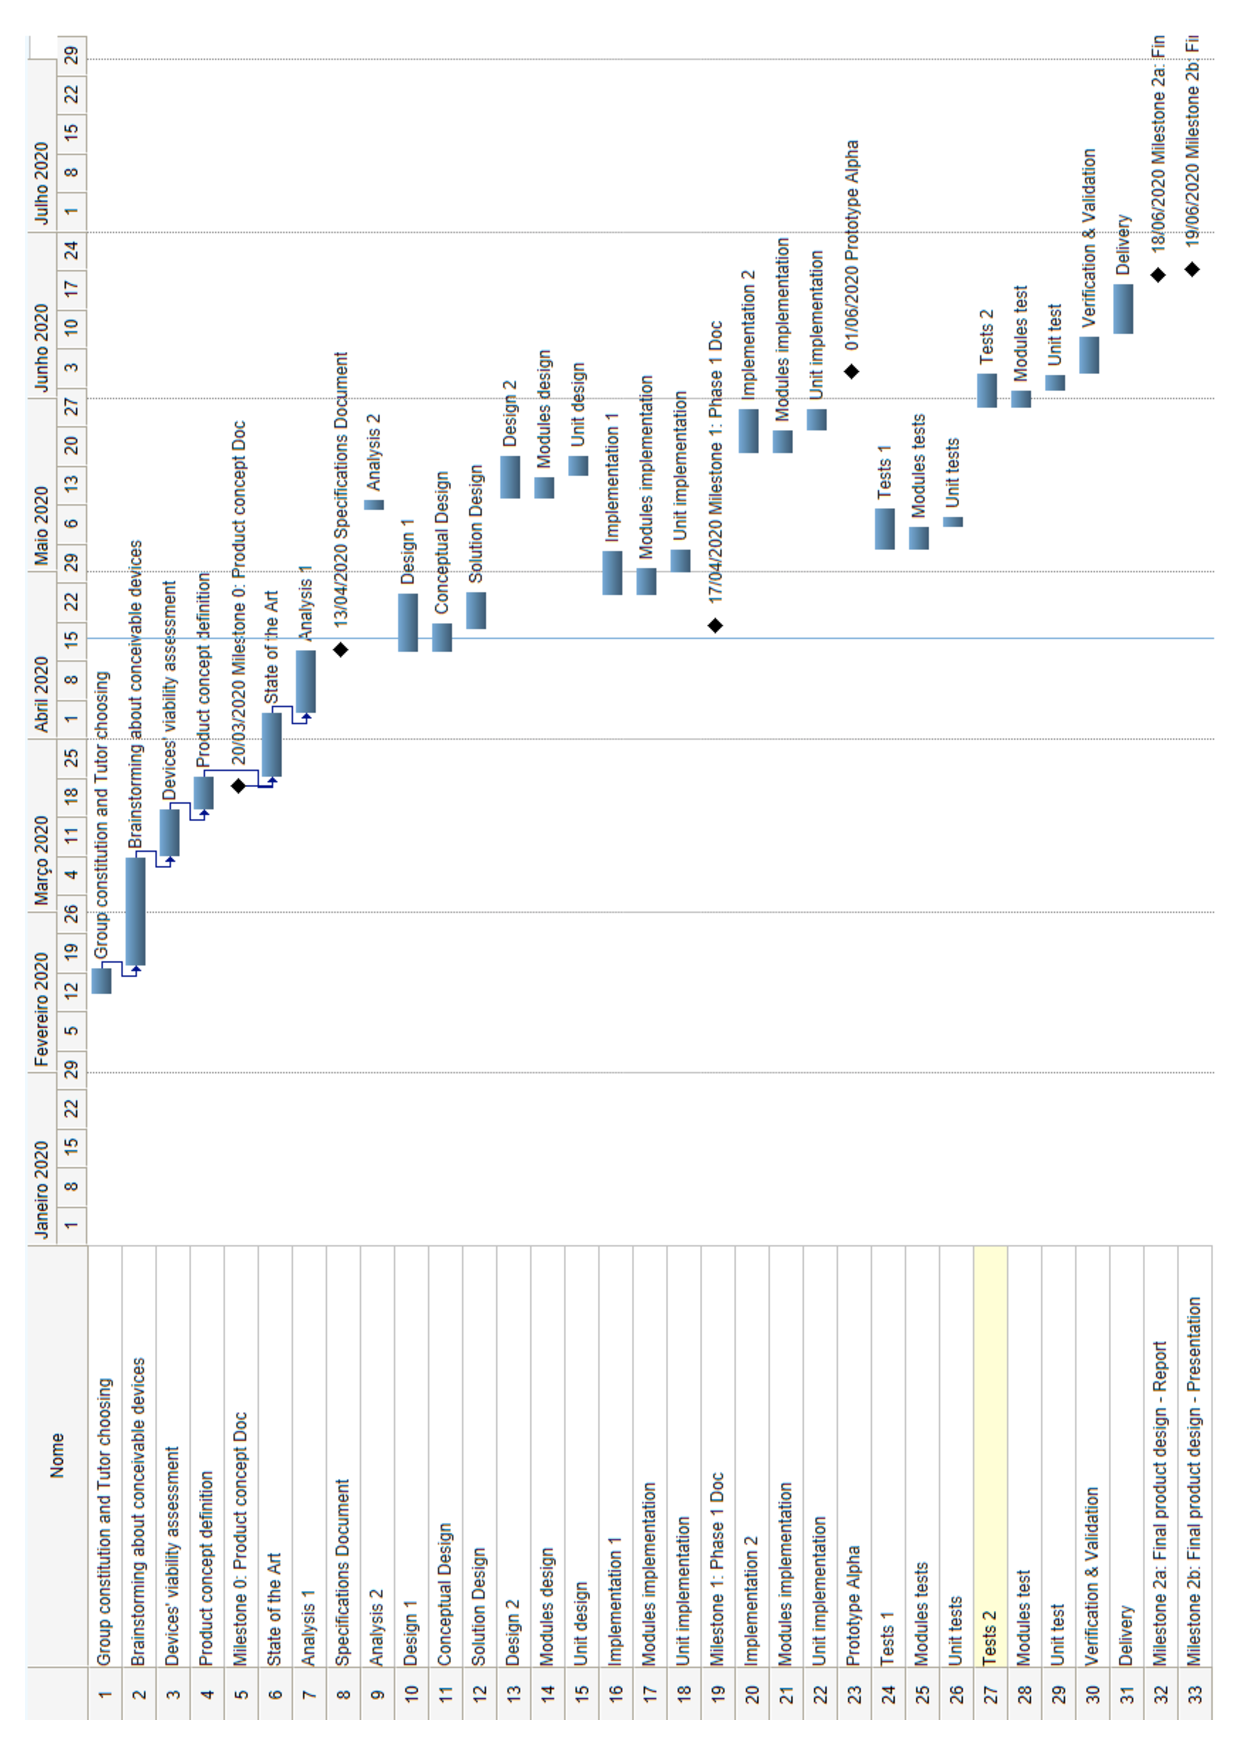
\includepdf[pages=-]{sec/pdf/gantt-diag-orig.pdf}
\begin{sidewaysfigure}[!h]
  \centering
  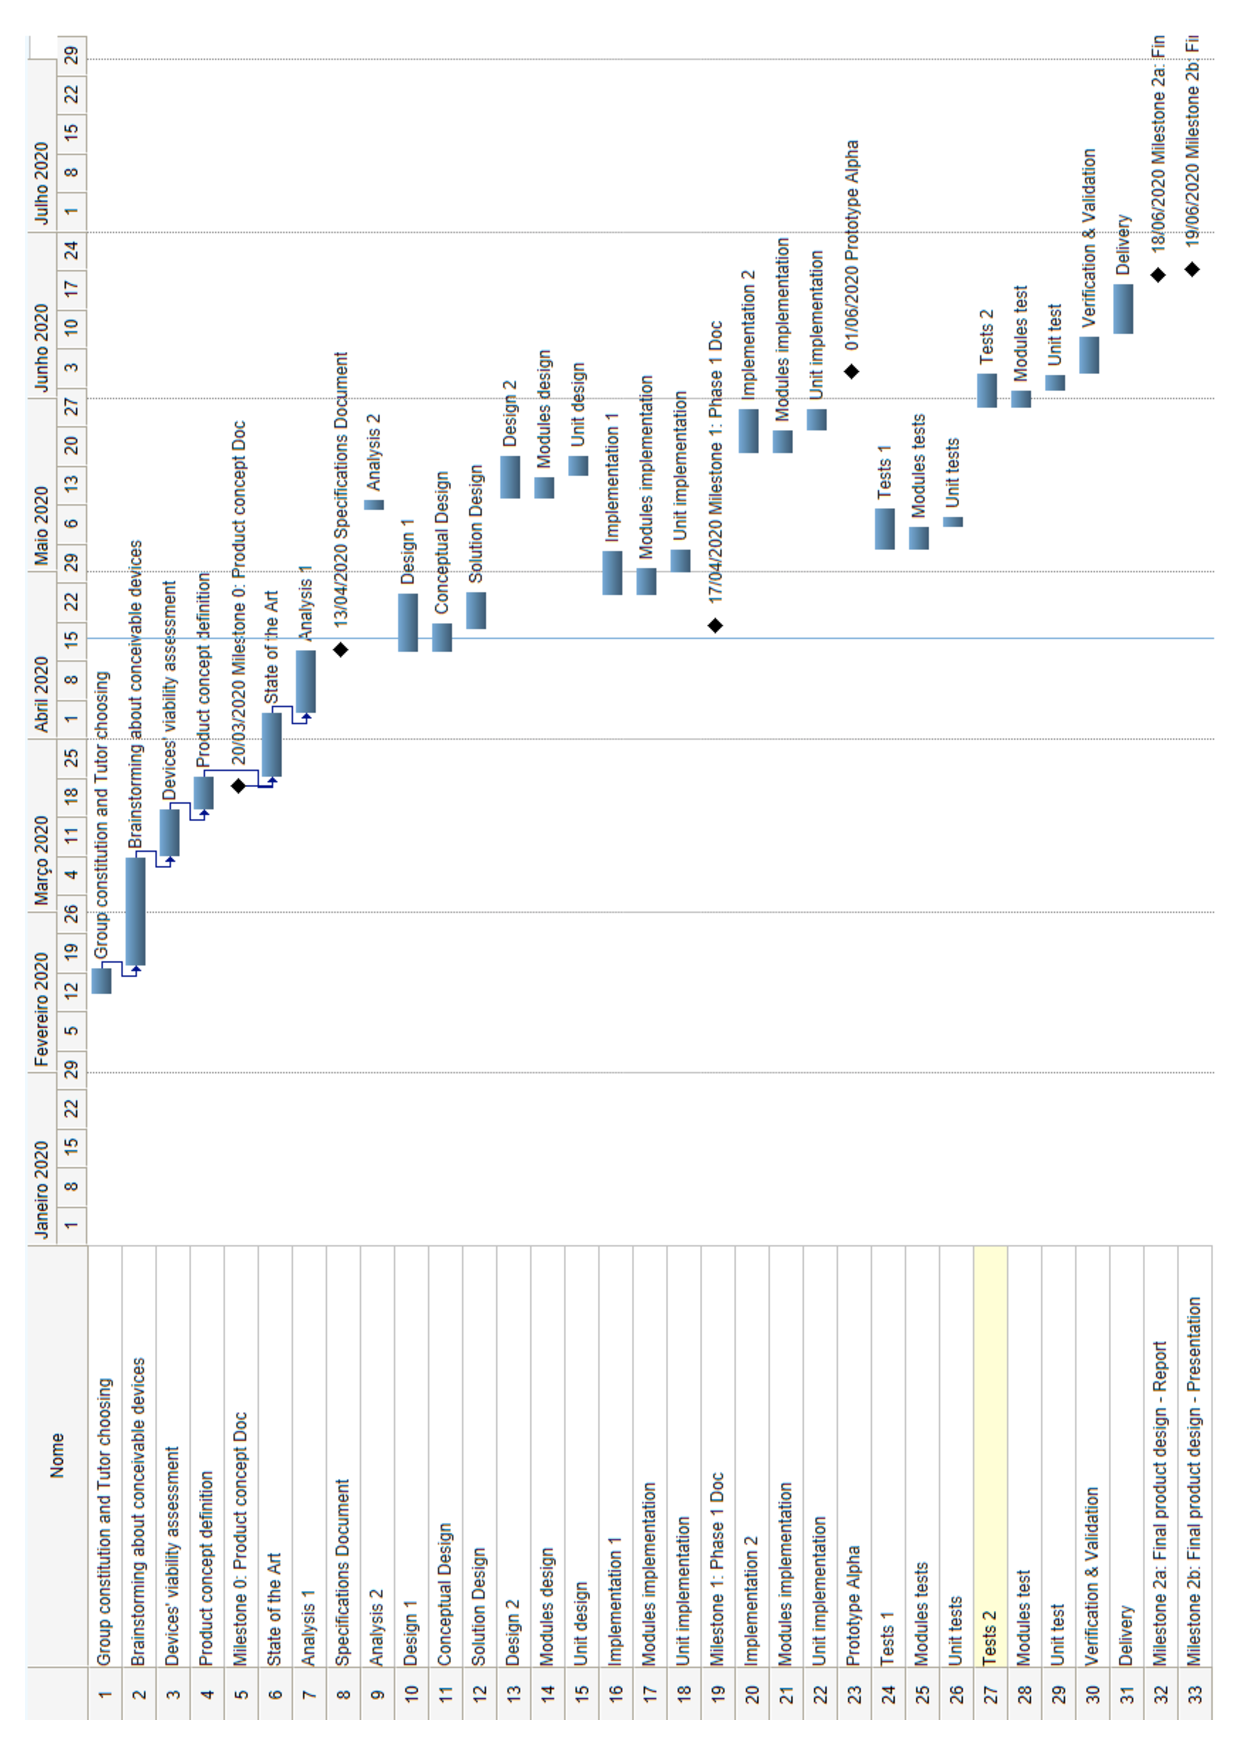
\includegraphics[page=1,width=1.0\textwidth]{sec/pdf/gantt-diag-orig.pdf} 
  \caption{Project planning --- Gantt diagram}%
  \label{fig:gantt-diag-orig}
\end{sidewaysfigure}
% 
%%% Local Variables:
%%% mode: latex
%%% TeX-master: "../Phase1"
%%% End:

\section{Tests}%
\label{sec:org3e2776f}
Tests are generally considered as those performed over any physical
component or prototype. Here, however, it is used in a broader sense, to reflect the tests
conducted into the system and the several prototypes, under the abnormal present
circumstances. The tests are divided into verification and validation tests.
\subsection{Verifications tests}%
\label{sec:orge9c79e2}
The verifications tests are tests performed internally by the design team to
check the compliance of the foreseen specifications. These tests are done after
the prototype alpha is concluded.

\subsubsection{Functionality}%
\label{sec:functionality}
The remotely operated vehicle is composed of several modules distributed along
several different platforms, some of which distanced from each other. In the
present abnormal circumstances, this is even more true. Thus, the proposed sets
of functionalities should be tested in the integrated system, by tracking and
analysing the user commands issued along the way until it finally reaches the
vehicle, assessing if it is correctly processed. For example, if the user issues
the vehicle to move to a given place, the message sent to the vehicle must be
signaled in each endpoint hit, and the vehicle should move to that place.

\subsubsection{Maximum Load}%
\label{sec:load}
The remotely controlled vehicle can be used in applications involving load
carrying (besides its own, obviously), e.g., packet delivery. For this purpose
it is important to determine the maximum load the vehicle can carry safely at
the minimum velocity defined. As the load increases, also increases the power
consumption, diminishing the autonomy. Thus, two alternative definitions, and
consequently, tests arise for the maximum load determination:
\begin{enumerate}
\item maximum load (at minimum velocity): maximum load the vehicle can carry
  safely at the minimum velocity defined.
\item maximum load (at 50\% over the mean power consumption): maximum load which
  causes a 50\% increase in the mean power consumption, i.e., while operating at
  mean velocity.
\end{enumerate}

To test the former, load should be increased slowly, measuring the vehicle
mean velocity, until the minimum velocity defined is achieved. To test the
latter, load should be increased slowly, measuring the power consumption, until
a 50\% increase over the mean power power consumption is detected, while
operating at the mean velocity.

\subsubsection{Autonomy}%
\label{sec:org532616f}
The vehicle is operated off-the-grid, thus, a portable power source must be
included. The autonomy --- time interval between battery fully charged and
safely discharged --- should be observed for the following scenarios:
\begin{enumerate}
\item No load and vehicle operating at maximum speed
\item No load and vehicle operating at mean speed
\item Maximum load and vehicle operating at maximum speed
\item Maximum load and vehicle operating at mean speed
\end{enumerate}
The autonomy is related to product's power consumption and the capacity of the
battery chosen. Under the present abnormal circumstances is not reasonable to
expect the product's power consumption to match the real one, thus, for all
purposes, this will be considered as the one drawn by the car module itself,
namely, the installed motors and sensors.

Then, the autonomy can be measured as
the time interval between battery fully charged and safely discharged (the car
stops), by fixating the car to a supporting structure with free moving wheels,
and imposing the aforementioned conditions.

\subsubsection{Velocity}%
\label{sec:org20789b4}
The vehicle must be operated within a safe range of velocity, while also not
increasing excessively the power consumption. Thus, these velocity boundaries
should be tested in the absence of an external load and in the presence of the
maximum load. It is important to define these boundaries as follows:
\begin{itemize}
\item minimum velocity: minimum velocity defined for the vehicle, which must be
  attained even in the condition of maximum load. This value must be selected to
  assure safe motor operation.
\item maximum velocity (no load): maximum velocity for the vehicle in the
  absence of an external load. This is the absolute maximum velocity for the
  vehicle.
\item maximum velocity (maximum load): maximum velocity for the vehicle in the
  presence of the maximum load. This value must be selected to prevent excessive
  power consumption and motor overheating.
\end{itemize}
The aforementioned velocities should be tested in the designed conditions,
within a sufficiently long distance to assure velocity reach and stabilization,
and compared to the ones provided in the foreseen specifications.

\subsubsection{Safety}%
\label{sec:orgf4c025f}
Safety is paramount in product design, especially considering the vehicle is to
be remotely operated. Safety can be analysed in two ways, considering the
preservation of people and goods. For the former, it is important to assure safe
user operation as well as safe human interaction --- the vehicle may encounter
several people along its path, but it must not inflict any damage. For the
latter, the vehicle under operating conditions must not inflict any damage to
goods.

To test human safety, it is important to identify the interactions between the
user and the product, and which are the most prevalent and dangerous. Even so,
the exhaustive test is outside the scope of the present work; a small set of
features will be tested accordingly to the devised user manual, containing the
safety measures. For example, battery installation and conditions should be
tested, eventually leading to the posterior incorporation of safety measures in
the product.

To test goods safety, it is reasonable to assume the operating conditions of the
vehicle. Under these it is important to consider the most critical ones that
concern the moments when the vehicle is left to be controlled locally, instead
of user controlled operation. The critical conditions for local operations are
divided into two sets:
\begin{itemize}
\item processing of user commands and vehicle operation: user commands can
  conflict with safety measures and, thus, should be overriden locally.
\item communication loss: the vehicle is left to odometric navigation,
  preserving the safety of people and goods.
\end{itemize}
To test these two scenarios, they should be replicated, observing the system
response and tolerance.%DONE

\subsubsection{Image acquisition}%
\label{sec:orgb1f5c2a}
The vehicle is equipped with a camera to assist the user in its navigation,
thus, requiring it to be feed to the user's platform within proper conditions.
The following variables are to be tested: frame rate, range, and resolution.

\paragraph{Frame rate}%
\label{sec:frame-rate-test}
The frame rate is the rate at which the user platform screen is updated with new
image information. It should be maintained within acceptable boundaries to serve
the purpose of assisting the user in the vehicle's navigation. To test it, the
number of frame displayed per second in the user screen must be updated and
checked against the defined boundaries.

\paragraph{Range}%
\label{sec:range-test}
The range is the maximum distance the camera can clearly effectively capture an
image without losing resolution. To test this, an object must be captured at
increasing distances, until the image resolution is lost.

\paragraph{Resolution}%
\label{sec:resolution-test}
The image resolution quantifies how close lines can be to each other and still
be visibly resolved, giving an information on the its detail. The minimum
resolution should be tested as providing the least amount of information
required for the user, while minimizing data transfer and processing overhead.

\subsubsection{Communication reliability}%
\label{sec:comm-reli}
A communication is reliable if it guarantees measures to deliver the data
conveyed in the communication link. As reliability imposes these measures, it
also adds overhead to the communication protocol, which must be considered
depending on the case. For example, for the devised product, an user command
must be acknowledged to be processed, otherwise, the user must be informed; on
the other hand, loosing frames from the video feed is not so critical --- user
can still observe conveniently the field of vision if the frame rate is within
acceptable boundaries. 

Thus, given the critical nature of user commands issued, the focus will be on
this communication link. To test the reliability dummy packets should be sent
from the user platform to the vehicle and be acknowledged and parsed correctly.

\subsubsection{Closed loop error (Control loops)}%
\label{sec:closed-loop-error}
The velocity, direction and distance to obstacles must be continuosly monitored
to ensure proper vehicle operation. The closed loop error must then be checked
mainly in three situations as a response to an user command:
\begin{itemize}
\item velocity: the user issued an command with a given mean velocity, which
  should be compared with the steady-state mean velocity of the vehicle. This
  can be tested by comparing the user defined velocity and the vehicle's;
\item direction: the user issued an command with a given direction, which should
  be compared to the vehicle direction. This can be tested by measuring the
  angle between final and initial points and comparing it with the user defined
  direction.
\item distance to obstacles: the user issued an command with a given direction
  and velocity which can cause it to crash. The local control must take over
  control, preventing this to happen, and the final distance to the obstacles
  must be assessed and compared to the defined one.
\end{itemize}

%An overshoot occurs when the output in a control system exceeds its final,
%steady state value generally caused by a sudden change in the system, in this
%case specifically, the placement of a load upon the conveyor will cause an
%overshoot in the latter’s velocity which must be controlled lest it cause
%problems.
%
%An overshoot will occur during the settling time, as such, using the same
%considerations taken in its measurement, it can be measured by observing the
%induced voltage at the generator (an overshoot in the conveyor’s velocity will
%correspond to a peak in the generator’s voltage).
%
%Using an oscilloscope to display the induced voltage at the generator and making
%use of the “single mode” present in these measuring instruments one can observe
%the change that will occur in the generator’s induced voltage, the peak voltage
%that will be seen when the load is placed upon the running conveyor is the
%electrical representation of the overshoot of velocity, then either by
%converting it to its physical representation or comparing it to the reference
%voltage one can arrive at a conclusion. It was agreed that the overshoot
%velocity should be \(V_{ss} \pm 10\%\), where \(V_{ss}\) is the stedy state
%velocity.

\subsection{Validation tests}%
\label{sec:orgff1a37d}
The validation tests should be performed by the client using the product’s
manual, so it is expected that a user without prior experience with the product
should be able to use it correctly and safely. On the present abnormal
circumstances, with limited access to the physical modules, specially for an
external agent, the validation is severely limited.
Thus, it should be limited to user interface validation.

For this purpose, an external agent will be provided with the software
application and the respective installation and usage manuals, and the feedback
will be collected and processed to further improve the product.
%%% Local Variables:
%%% mode: latex
%%% TeX-master: "../Phase1"
%%% End:

\section{Initial design}%
\label{sec:org68fdd80}

Following an analysis of the product’s family tree (remote controlled cars) and the state of the art, an initial design of the product itself can be produced (fig.~\ref{fig:initial-design}).
The selected approach was top-down, in the sense that the requirements and specifications were addressed and that resulted in a general diagram of the product concept. Some macro-level decisions were made in this stage to narrow the problem’s solutions pool, as follows:

\begin{itemize}
\item  The car itself should be battery-powered, as it is a free-moving object that is intended to work in environments where trailing cables could interfere with its regular movement.

\item The device used to control the car should ideally be one already owned by the user, with an integrated screen (e.g. smartphone), as it would make it more affordable and have a more straightforward interface.

\item The protocol for communication between the controlling device and the Rover should be chosen from within the pool of those readily available to smartphones (e.g. Wi-Fi, GPRS) to keep the price of the overall product down and make it as practical as possible.

\item  The control and communication unit for the car should be divided into two modules: one which can interface directly with the camera module and manage data transmission and reception at the applicational level of the TCP/IP protocol stack, with enough throughput for the specified video resolution and framerate. And another one which can measure and process sensor inputs and control the actuators in real-time.

\end{itemize}

\begin{figure}[!ht]
\centering
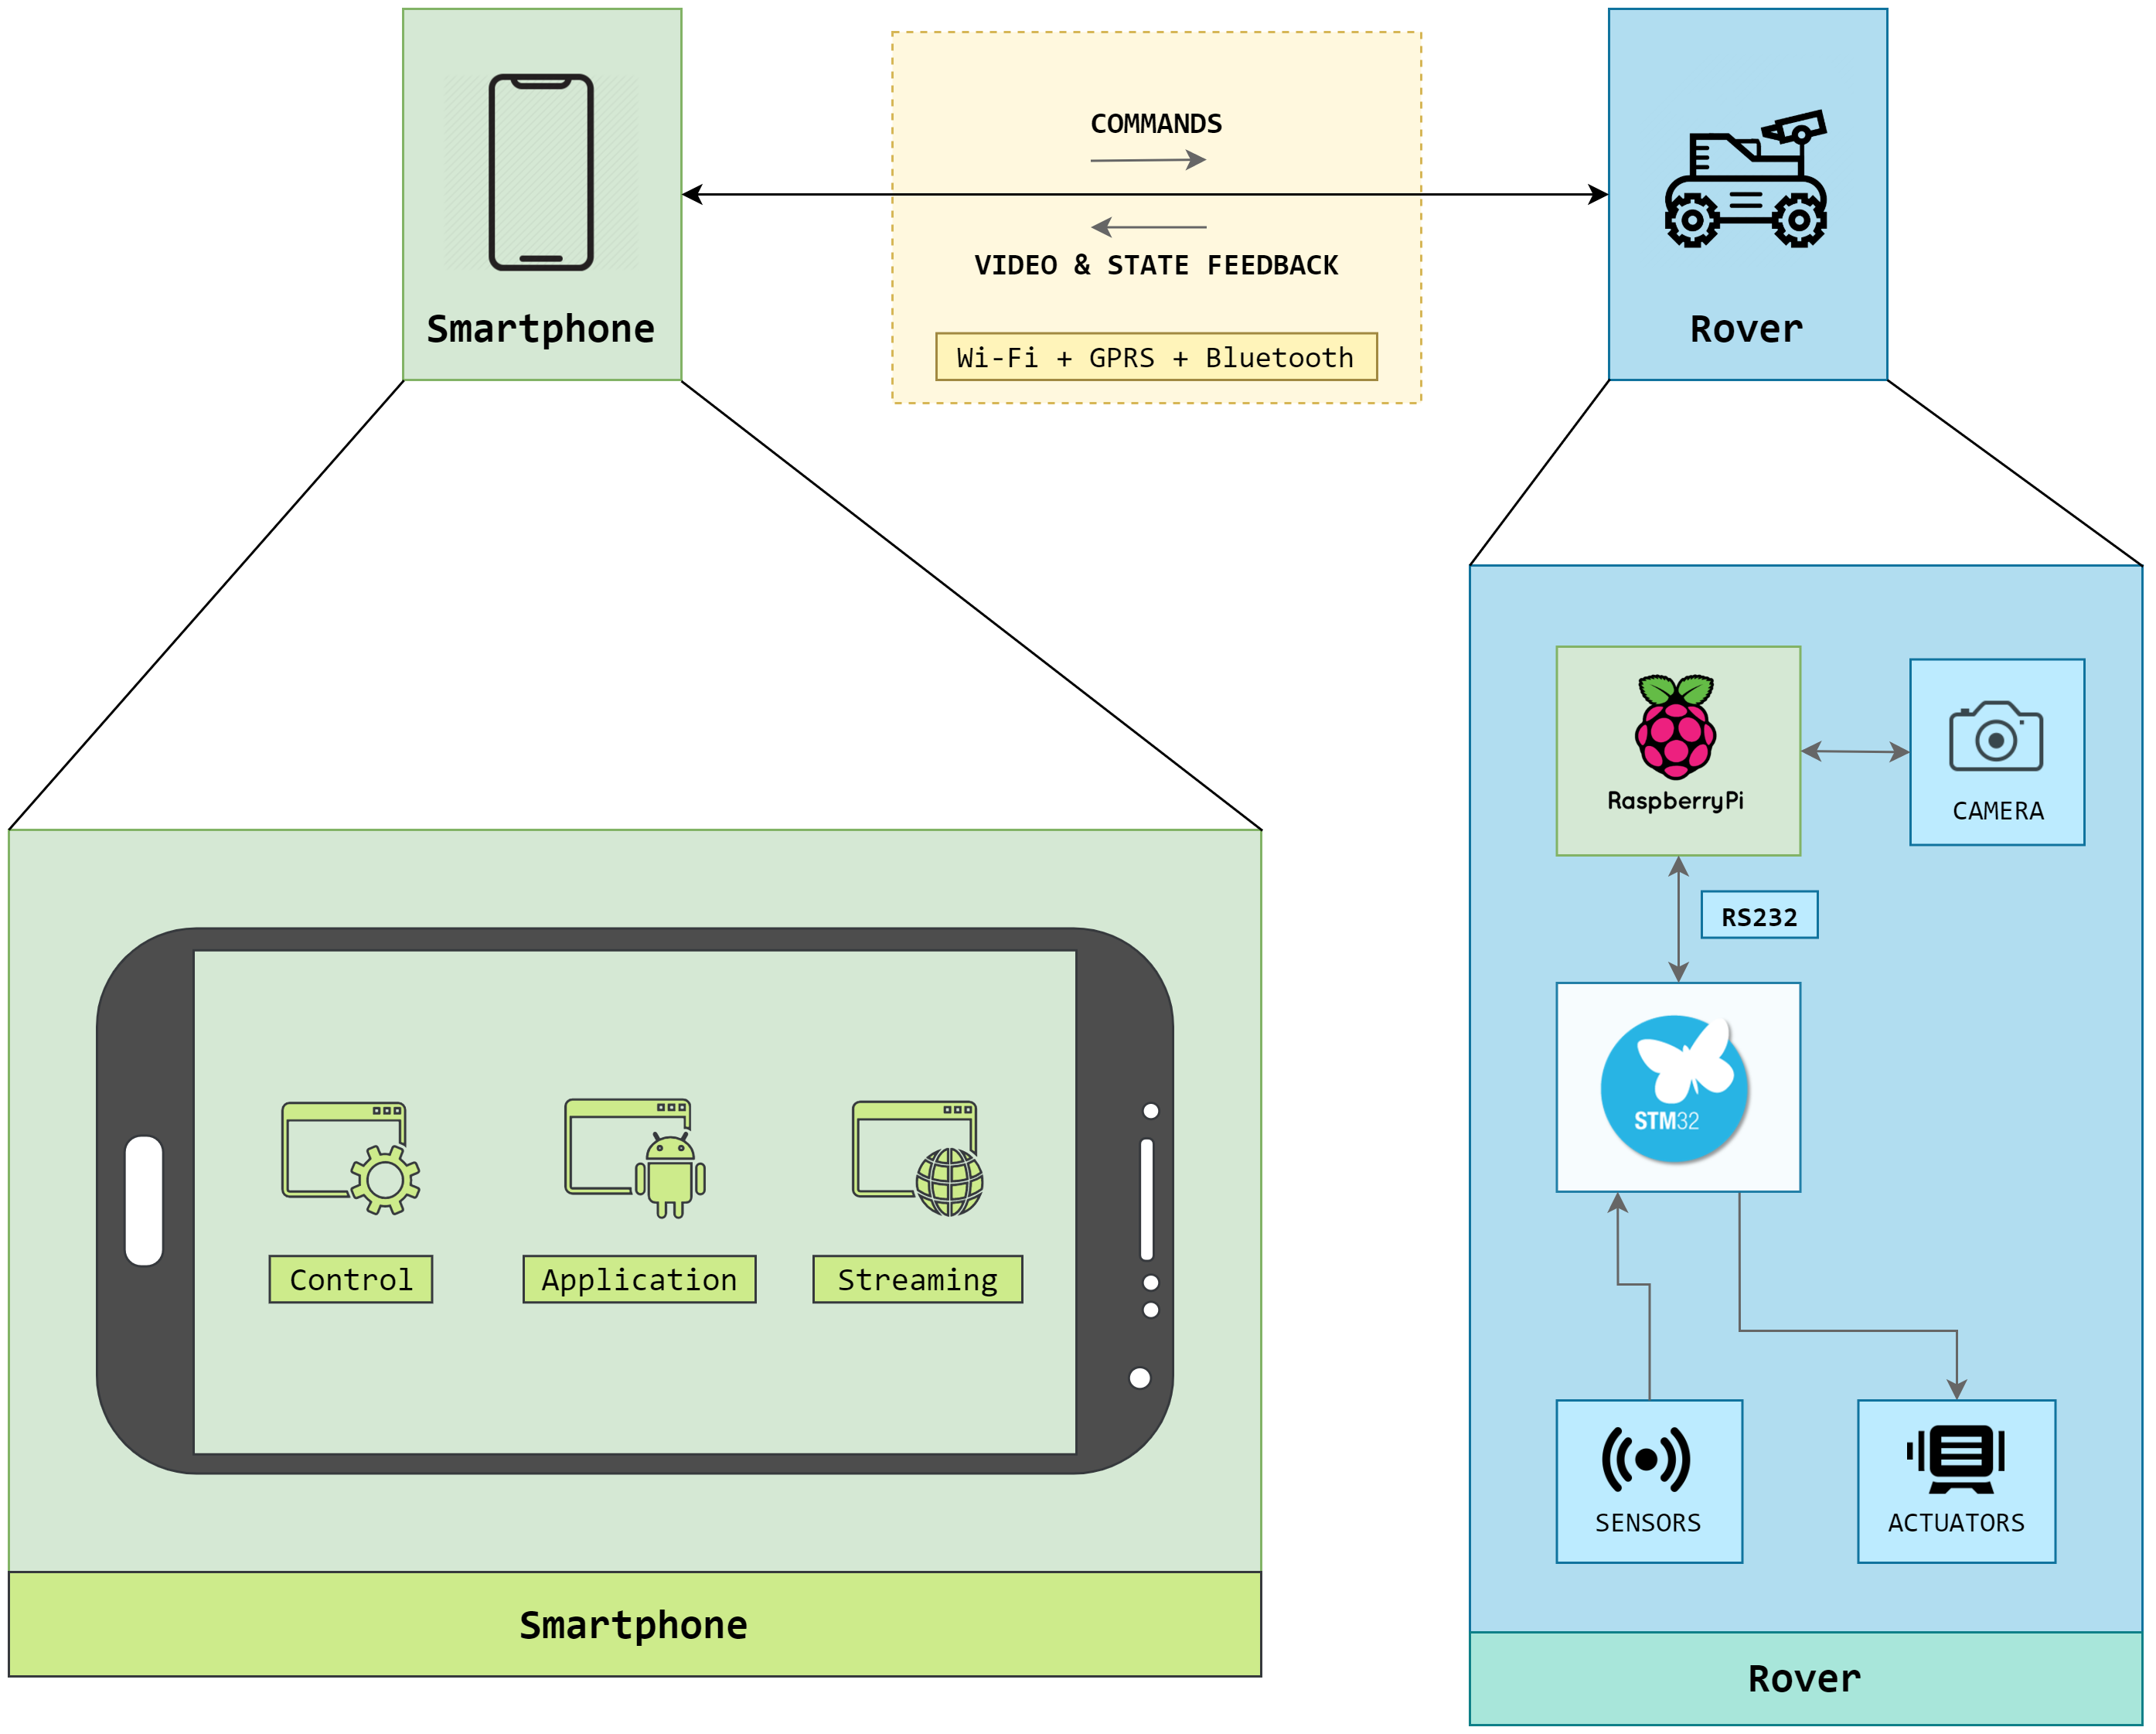
\includegraphics[width=1.0\textwidth]{./sec/img/initial_design_diagram.png}
\caption{\label{fig:initial-design}Initial design: Block diagram view}
\end{figure}

Thus, summarising, the initial design yields the system illustrated in
fig.~\ref{fig:initial-design}, comprised of:

\begin{itemize}
\item \textbf{ Raspberry Pi}: Interfaces with the camera directly, transmitting the information it receives to the smartphone. Receives user commands and sends sensorial information back to it;

\item \textbf{STM32}: Sends sensorial information to the Raspberry Pi module and receives commands from it. Controls the actuators according to the given instructions and sensor readings;

\item \textbf{Actuators}: DC Motors that control the car´s movement and headlights for nocturnal or low light conditions;

\item \textbf{Sensors}: Odometric sensors that support the detection of obstacles and luminosity sensors;

\item \textbf{Camera}: Device connected to the Raspberry Pi that allows the live stream of the car´s surrounding environment;

\item \textbf{Smartphone}: Grant visual feedback from the camera´s live feed also allowing the user to control the movement of the vehicle intuitively;

\end{itemize}

%%% Local Variables:
%%% mode: latex
%%% TeX-master: "../Phase1"
%%% End:
\end{document}